\documentclass[11pt, a4paper]{article}
\usepackage{pdfpages}
\usepackage{parallel}
\usepackage[T2A]{fontenc}
\usepackage{ucs}
\usepackage[utf8x]{inputenc}
\usepackage[polish,english,russian]{babel}
\usepackage{hyperref}
\usepackage{rotating}
\usepackage[inner=2cm,top=1.8cm,outer=2cm,bottom=2.3cm,nohead]{geometry}
\usepackage{listings}
\usepackage{graphicx}
\usepackage{wrapfig}
\usepackage{longtable}
\usepackage{indentfirst}
\usepackage{array}
\usepackage{tikzsymbols}
\usepackage{soul}
\usepackage[ruled,vlined]{algorithm2e}
%\counterwithout{figure}{section} 

\usepackage{url}
\makeatletter
\g@addto@macro{\UrlBreaks}{\UrlOrds}
\makeatother

\newcolumntype{P}[1]{>{\raggedright\arraybackslash}p{#1}}
\frenchspacing
\usepackage{fixltx2e} %text sub- and superscripts
\usepackage{icomma} % коскі ў матэматычным рэжыме
\PreloadUnicodePage{4}

\newcommand{\longpage}{\enlargethispage{\baselineskip}}
\newcommand{\shortpage}{\enlargethispage{-\baselineskip}}

\def\switchlang#1{\expandafter\csname switchlang#1\endcsname}
\def\switchlangbe{
\let\saverefname=\refname%
\def\refname{Літаратура}%
\def\figurename{Іл.}%
}
\def\switchlangen{
\let\saverefname=\refname%
\def\refname{References}%
\def\figurename{Fig.}%
}
\def\switchlangru{
\let\saverefname=\refname%
\let\savefigurename=\figurename%
\def\refname{Литература}%
\def\figurename{Рис.}%
}

\hyphenation{admi-ni-stra-tive}
\hyphenation{ex-pe-ri-ence}
\hyphenation{fle-xi-bi-li-ty}
\hyphenation{Py-thon}
\hyphenation{ma-the-ma-ti-cal}
\hyphenation{re-ported}
\hyphenation{imp-le-menta-tions}
\hyphenation{pro-vides}
\hyphenation{en-gi-neering}
\hyphenation{com-pa-ti-bi-li-ty}
\hyphenation{im-pos-sible}
\hyphenation{desk-top}
\hyphenation{elec-tro-nic}
\hyphenation{com-pa-ny}
\hyphenation{de-ve-lop-ment}
\hyphenation{de-ve-loping}
\hyphenation{de-ve-lop}
\hyphenation{da-ta-ba-se}
\hyphenation{plat-forms}
\hyphenation{or-ga-ni-za-tion}
\hyphenation{pro-gramming}
\hyphenation{in-stru-ments}
\hyphenation{Li-nux}
\hyphenation{sour-ce}
\hyphenation{en-vi-ron-ment}
\hyphenation{Te-le-pathy}
\hyphenation{Li-nux-ov-ka}
\hyphenation{Open-BSD}
\hyphenation{Free-BSD}
\hyphenation{men-ti-on-ed}
\hyphenation{app-li-ca-tion}

\def\progref!#1!{\texttt{#1}}
\renewcommand{\arraystretch}{2} %Іначай формулы ў матрыцы зліпаюцца з лініямі
\usepackage{array}

\def\interview #1 (#2), #3, #4, #5\par{

\section[#1, #3, #4]{#1 -- #3, #4}
\def\qname{LVEE}
\def\aname{#1}
\def\q ##1\par{{\noindent \bf \qname: ##1 }\par}
\def\a{{\noindent \bf \aname: } \def\qname{L}\def\aname{#2}}
}

\def\interview* #1 (#2), #3, #4, #5\par{

\section*{#1\\{\small\rm #3, #4. #5}}
\ifx\ParallelWhichBox\undefined%
    \addcontentsline{toc}{section}{#1, #3, #4}%
\else%
\ifnum\ParallelWhichBox=0%
    \addcontentsline{toc}{section}{#1, #3, #4}%
\fi\fi%

\def\qname{LVEE}
\def\aname{#1}
\def\q ##1\par{{\noindent \bf \qname: ##1 }\par}
\def\a{{\noindent \bf \aname: } \def\qname{L}\def\aname{#2}}
}

\newcommand{\interviewfooter}[1]{
\vskip 1em
\noindent \textit{#1}
}


\begin{document}

\title{1999 "--- Trackerball ProTrack 60i trackball}
\date{}
\maketitle

ProTrack 60i произведен фирмой Trackerball "--- обретшим в 1995 году самостоятельность
бывшим подразделением компании Marconi - разработчика самого первого трекбола для радарной установки в 1940-х годах для управления экранным курсором военных радаров \cite{history}.

\begin{figure}[h]
    \centering
    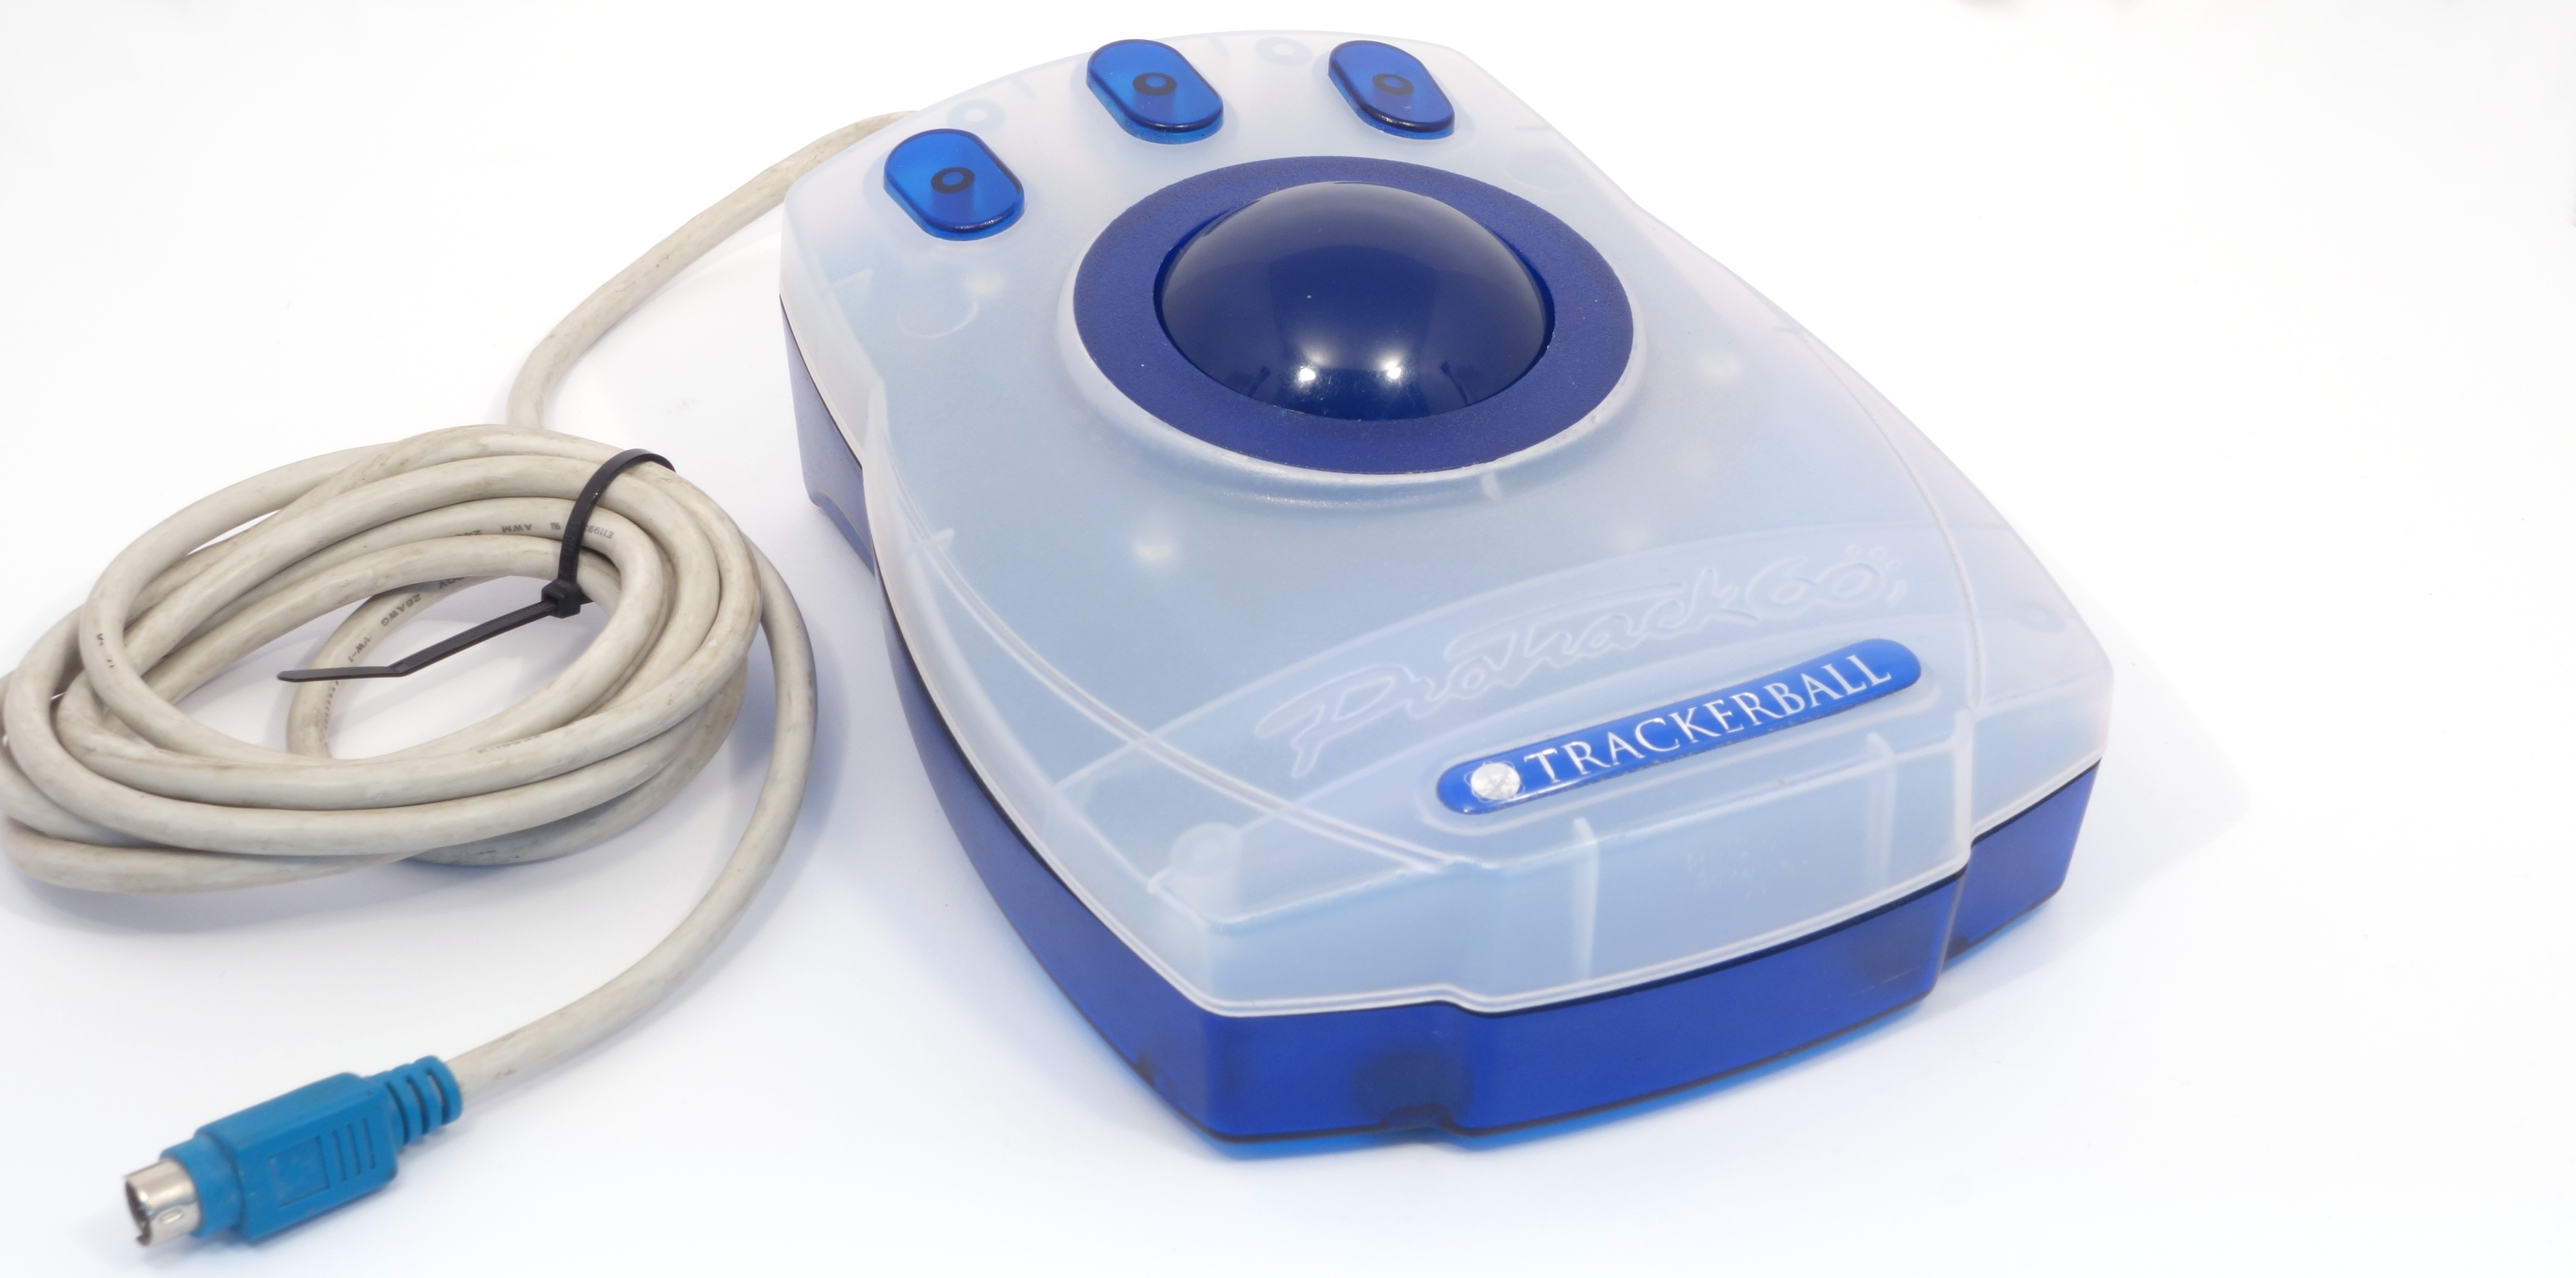
\includegraphics[scale=0.3]{1999_protrack_60i/monstr1_30.jpg}
    \caption{Трекбол ProTrack 60i}
    \label{fig:ProTrack60i}
\end{figure}

Трекбол выпускался в двух модификациях: R60 (ProTrack 60) с характерной расцветкой "--- белый корпус с черным шаром и кнопками, и R60i (ProTrack 60i) с полупрозрачным корпусом и синим шаром с подсветкой, предназначенной для использования в слабоосвещенных помещениях, которая показанна на рис. \ref{fig:ProTrack60i}. Наиболее распространенными интерфейсами подключения являются PS/2 и USB, однако на сайте компании Cursor Controls, в состав которой Trackerball вошла в 2000 году,  также упоминаются интерфейсы RS232, SUN и DEC \cite{cursorcontrols}.

Заметим, что данное устройство является чрезвычайно габаритным трекболом (рис. \ref{fig:ProTrack60iSize}). Диаметр шара составляет 63,5 мм (2.5 дюйма).

\begin{figure}[h]
    \centering
    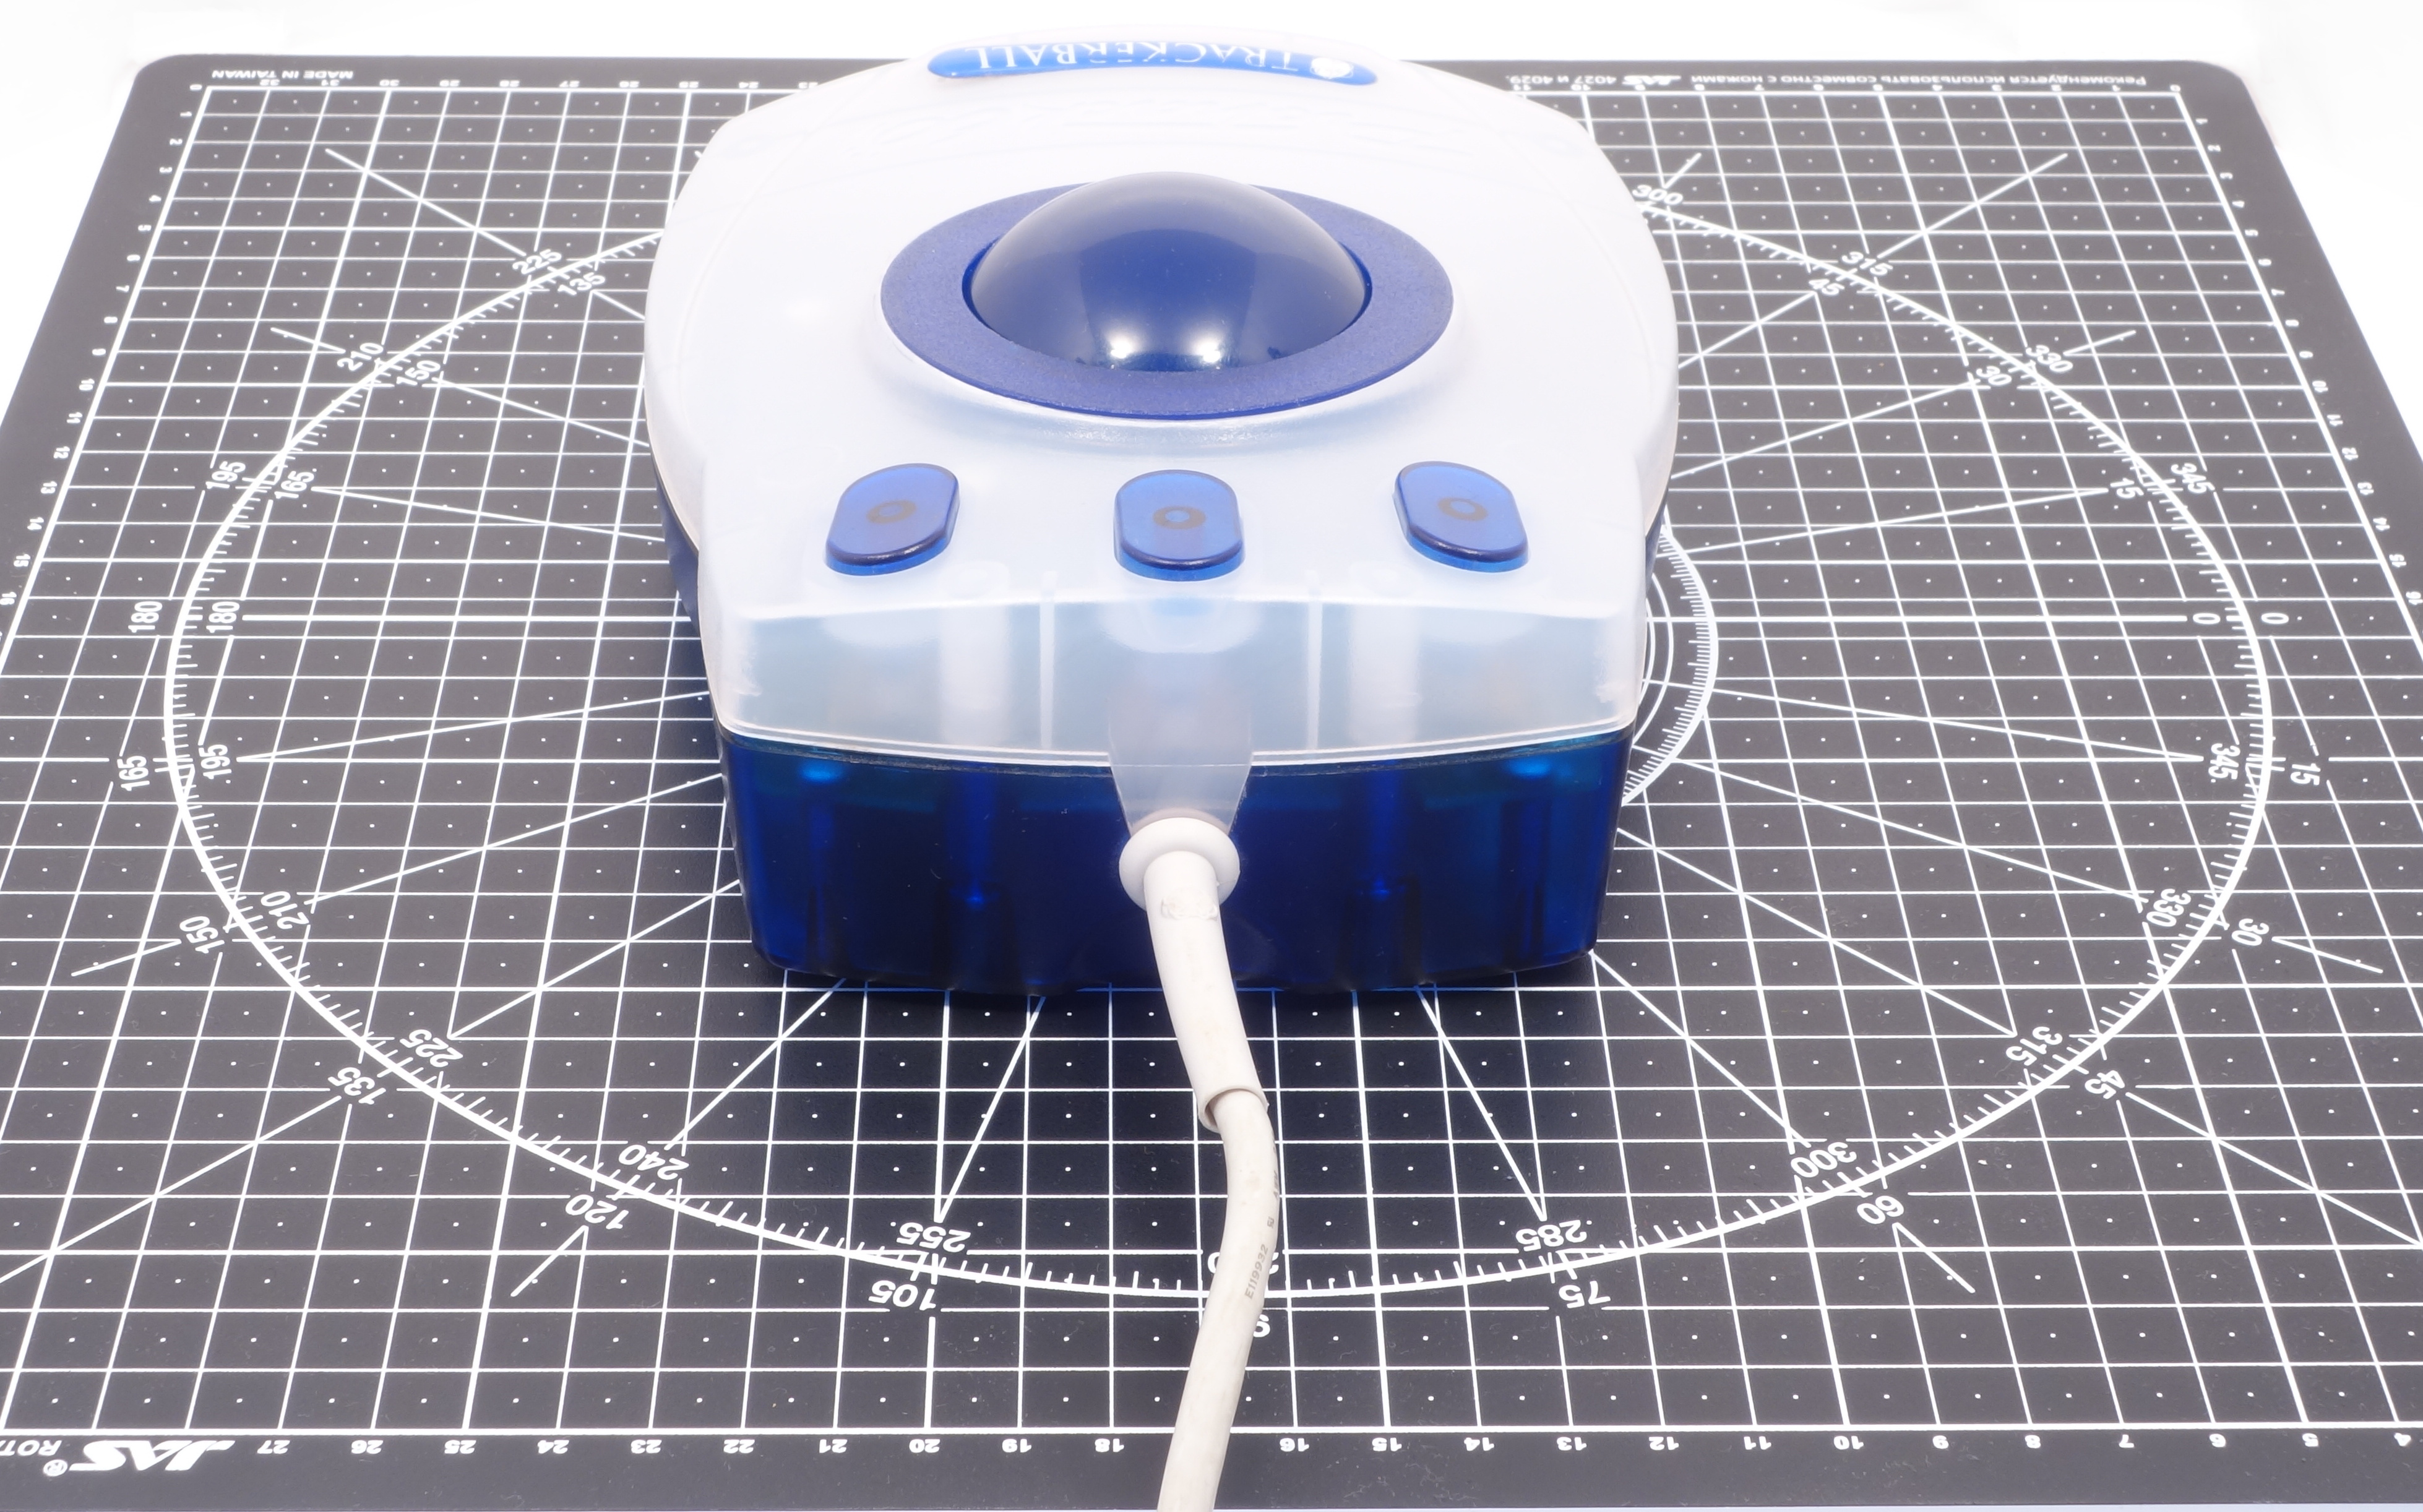
\includegraphics[scale=0.3]{1999_protrack_60i/monstr2.jpg}
    \caption{Изображение ProTrack 60i на размерном коврике с шагом сетки 1~см}
    \label{fig:ProTrack60iSize}
\end{figure}

Трекбол оснащён тремя кнопками, расположенными с противоположной от пользователя стороны, за шаром.
Согласно предположению, сделанному в \cite{trackballfan}, такое расположение кнопок минимизирует вероятность их случайного нажатия при перемещении шара, что очевидно является важным при использовании трекбола в индустриальных либо военных установках, но несколько затрудняет операцию перетаскивания (не характерную для подобного применения).
Трекбол не имеет колеса прокрутки, однако документация производителя упоминает возможность скроллинга шаром, которая активируется и деактивируется нажатиями на среднюю кнопку.

\begin{figure}[h]
    \centering
    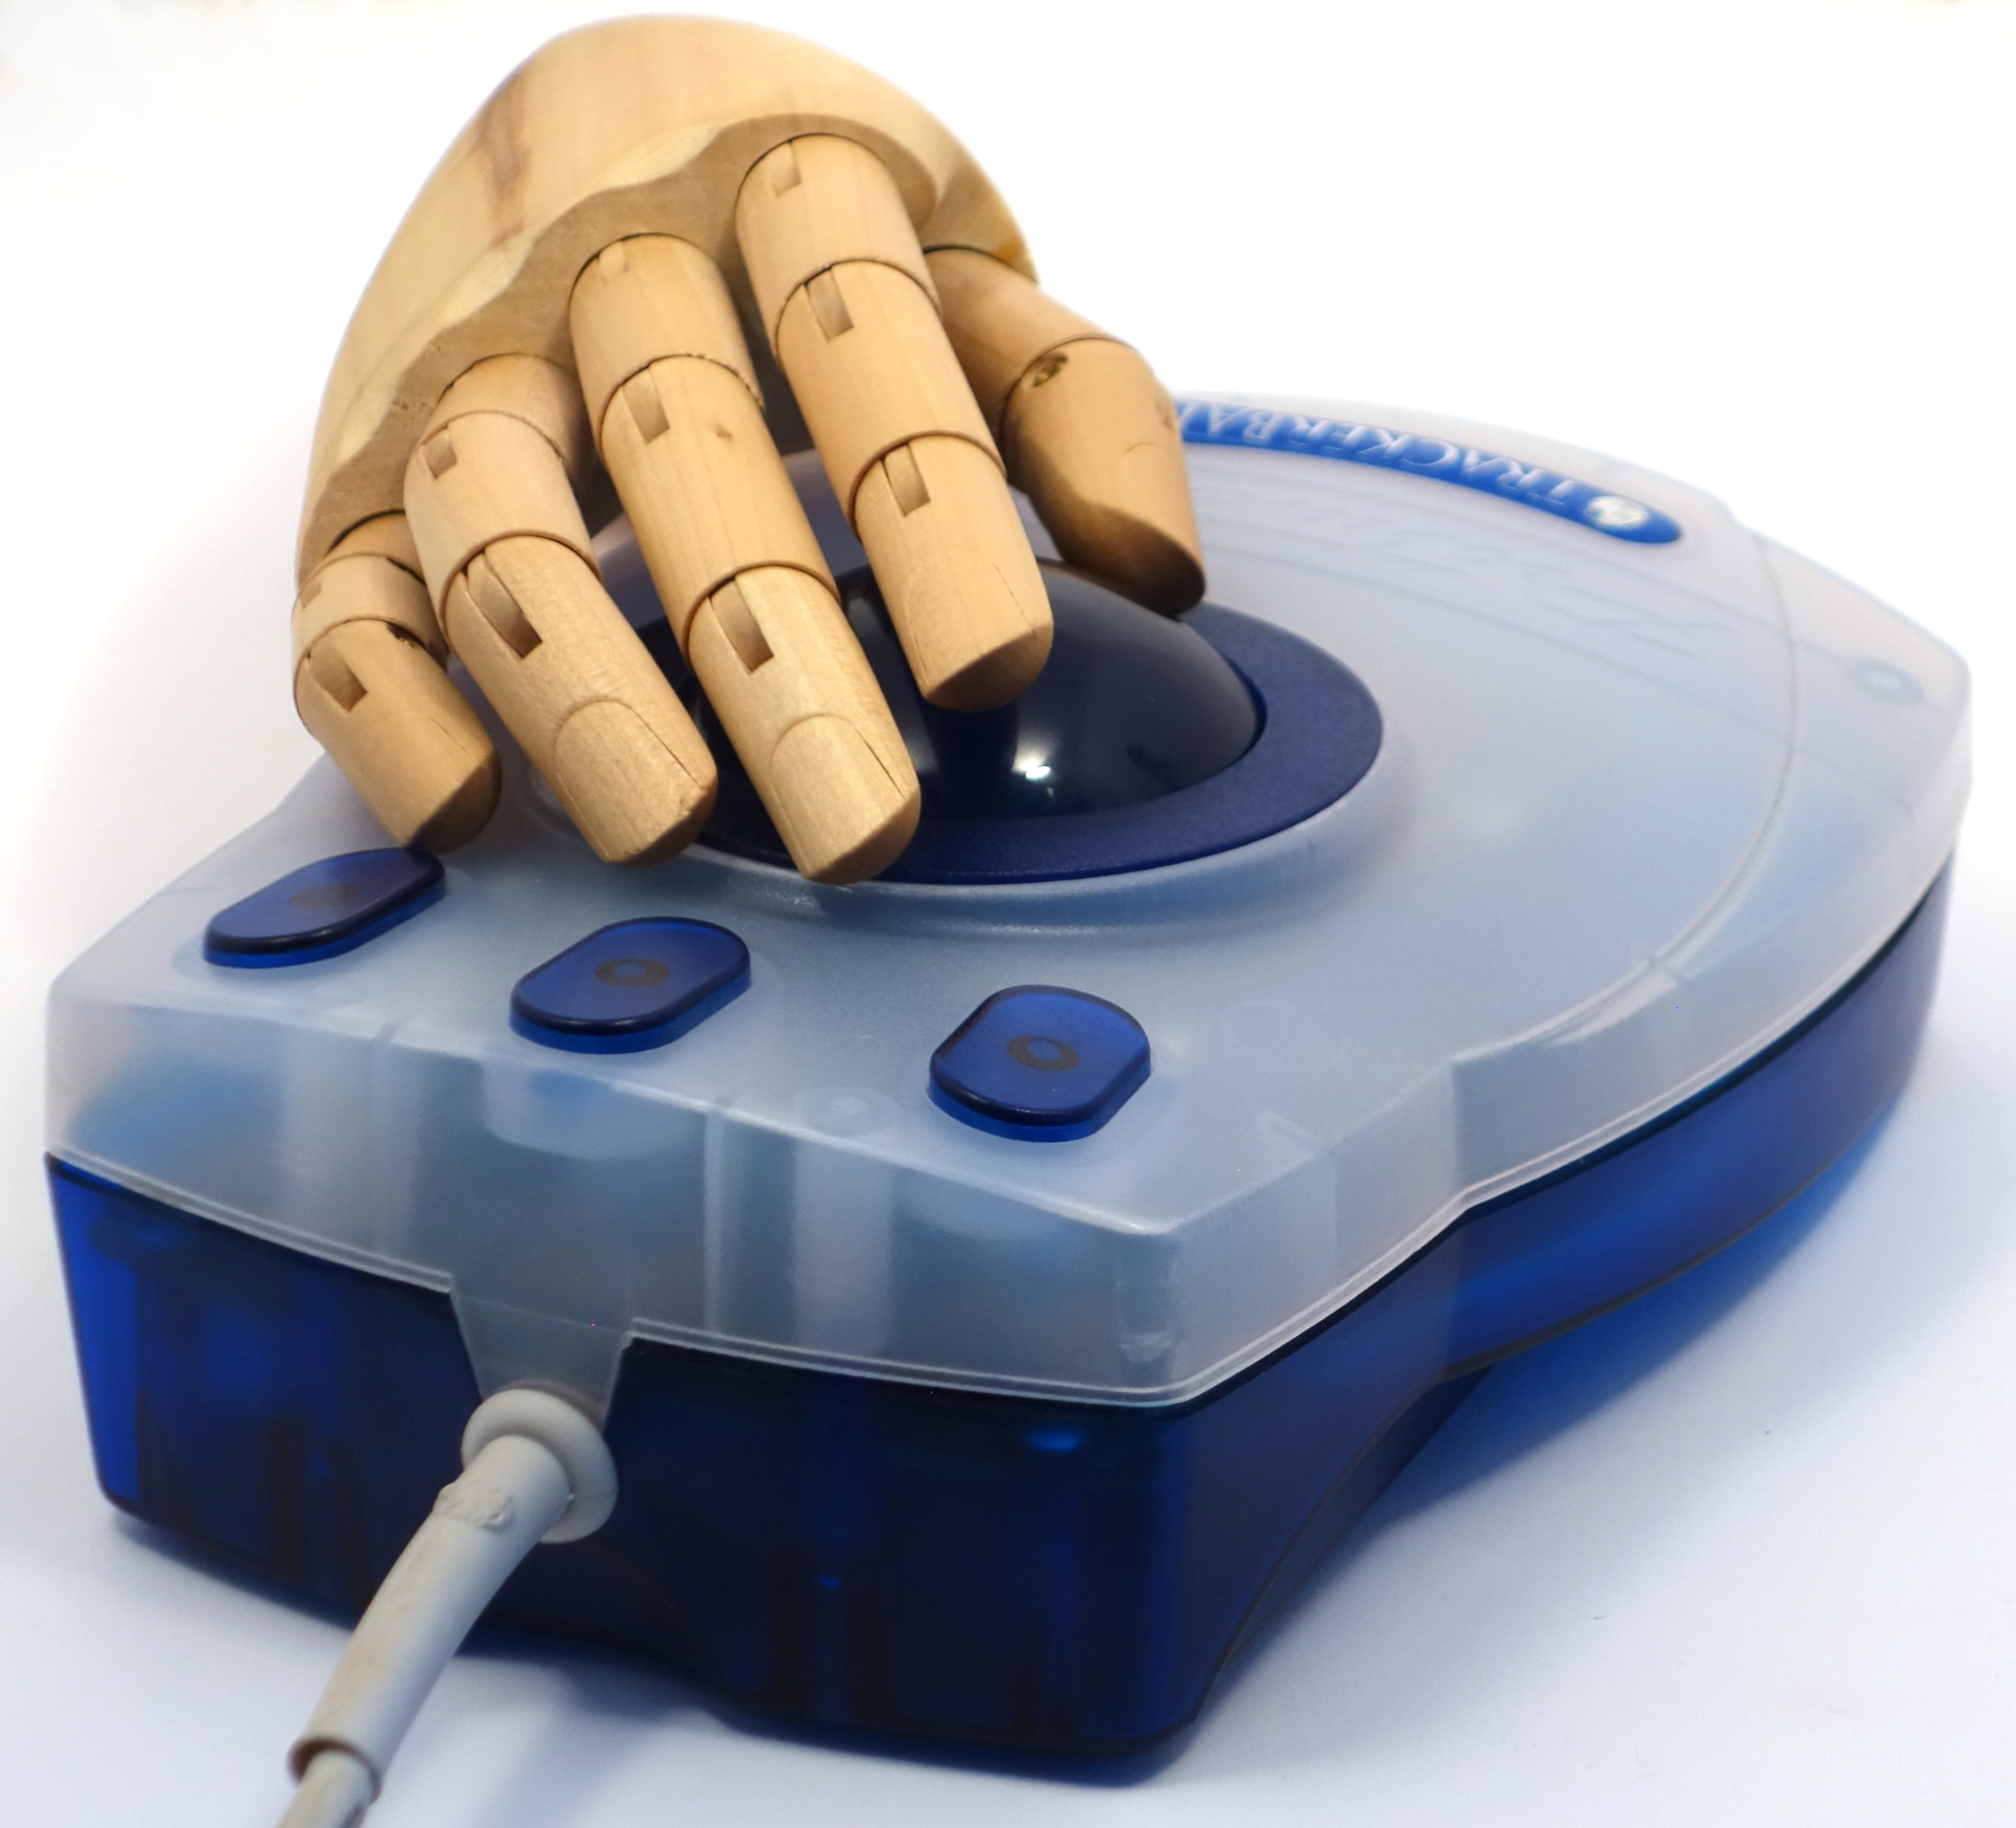
\includegraphics[scale=0.3]{1999_protrack_60i/raz_monstr_60.jpg}
    \caption{Изображение ProTrack 60i с моделью руки человека}
    \label{fig:ProTrack60iHand}
\end{figure}

На рис. \ref{fig:ProTrack60iTopBottom} можно видеть верхнюю и нижнюю стороны трекбола.
На верхней части корпуса присутствует рельефная надпись ProTrack 60i, а также эмблема с надписью <<TRACKERBALL>>.

\begin{figure}[h]
    \centering
    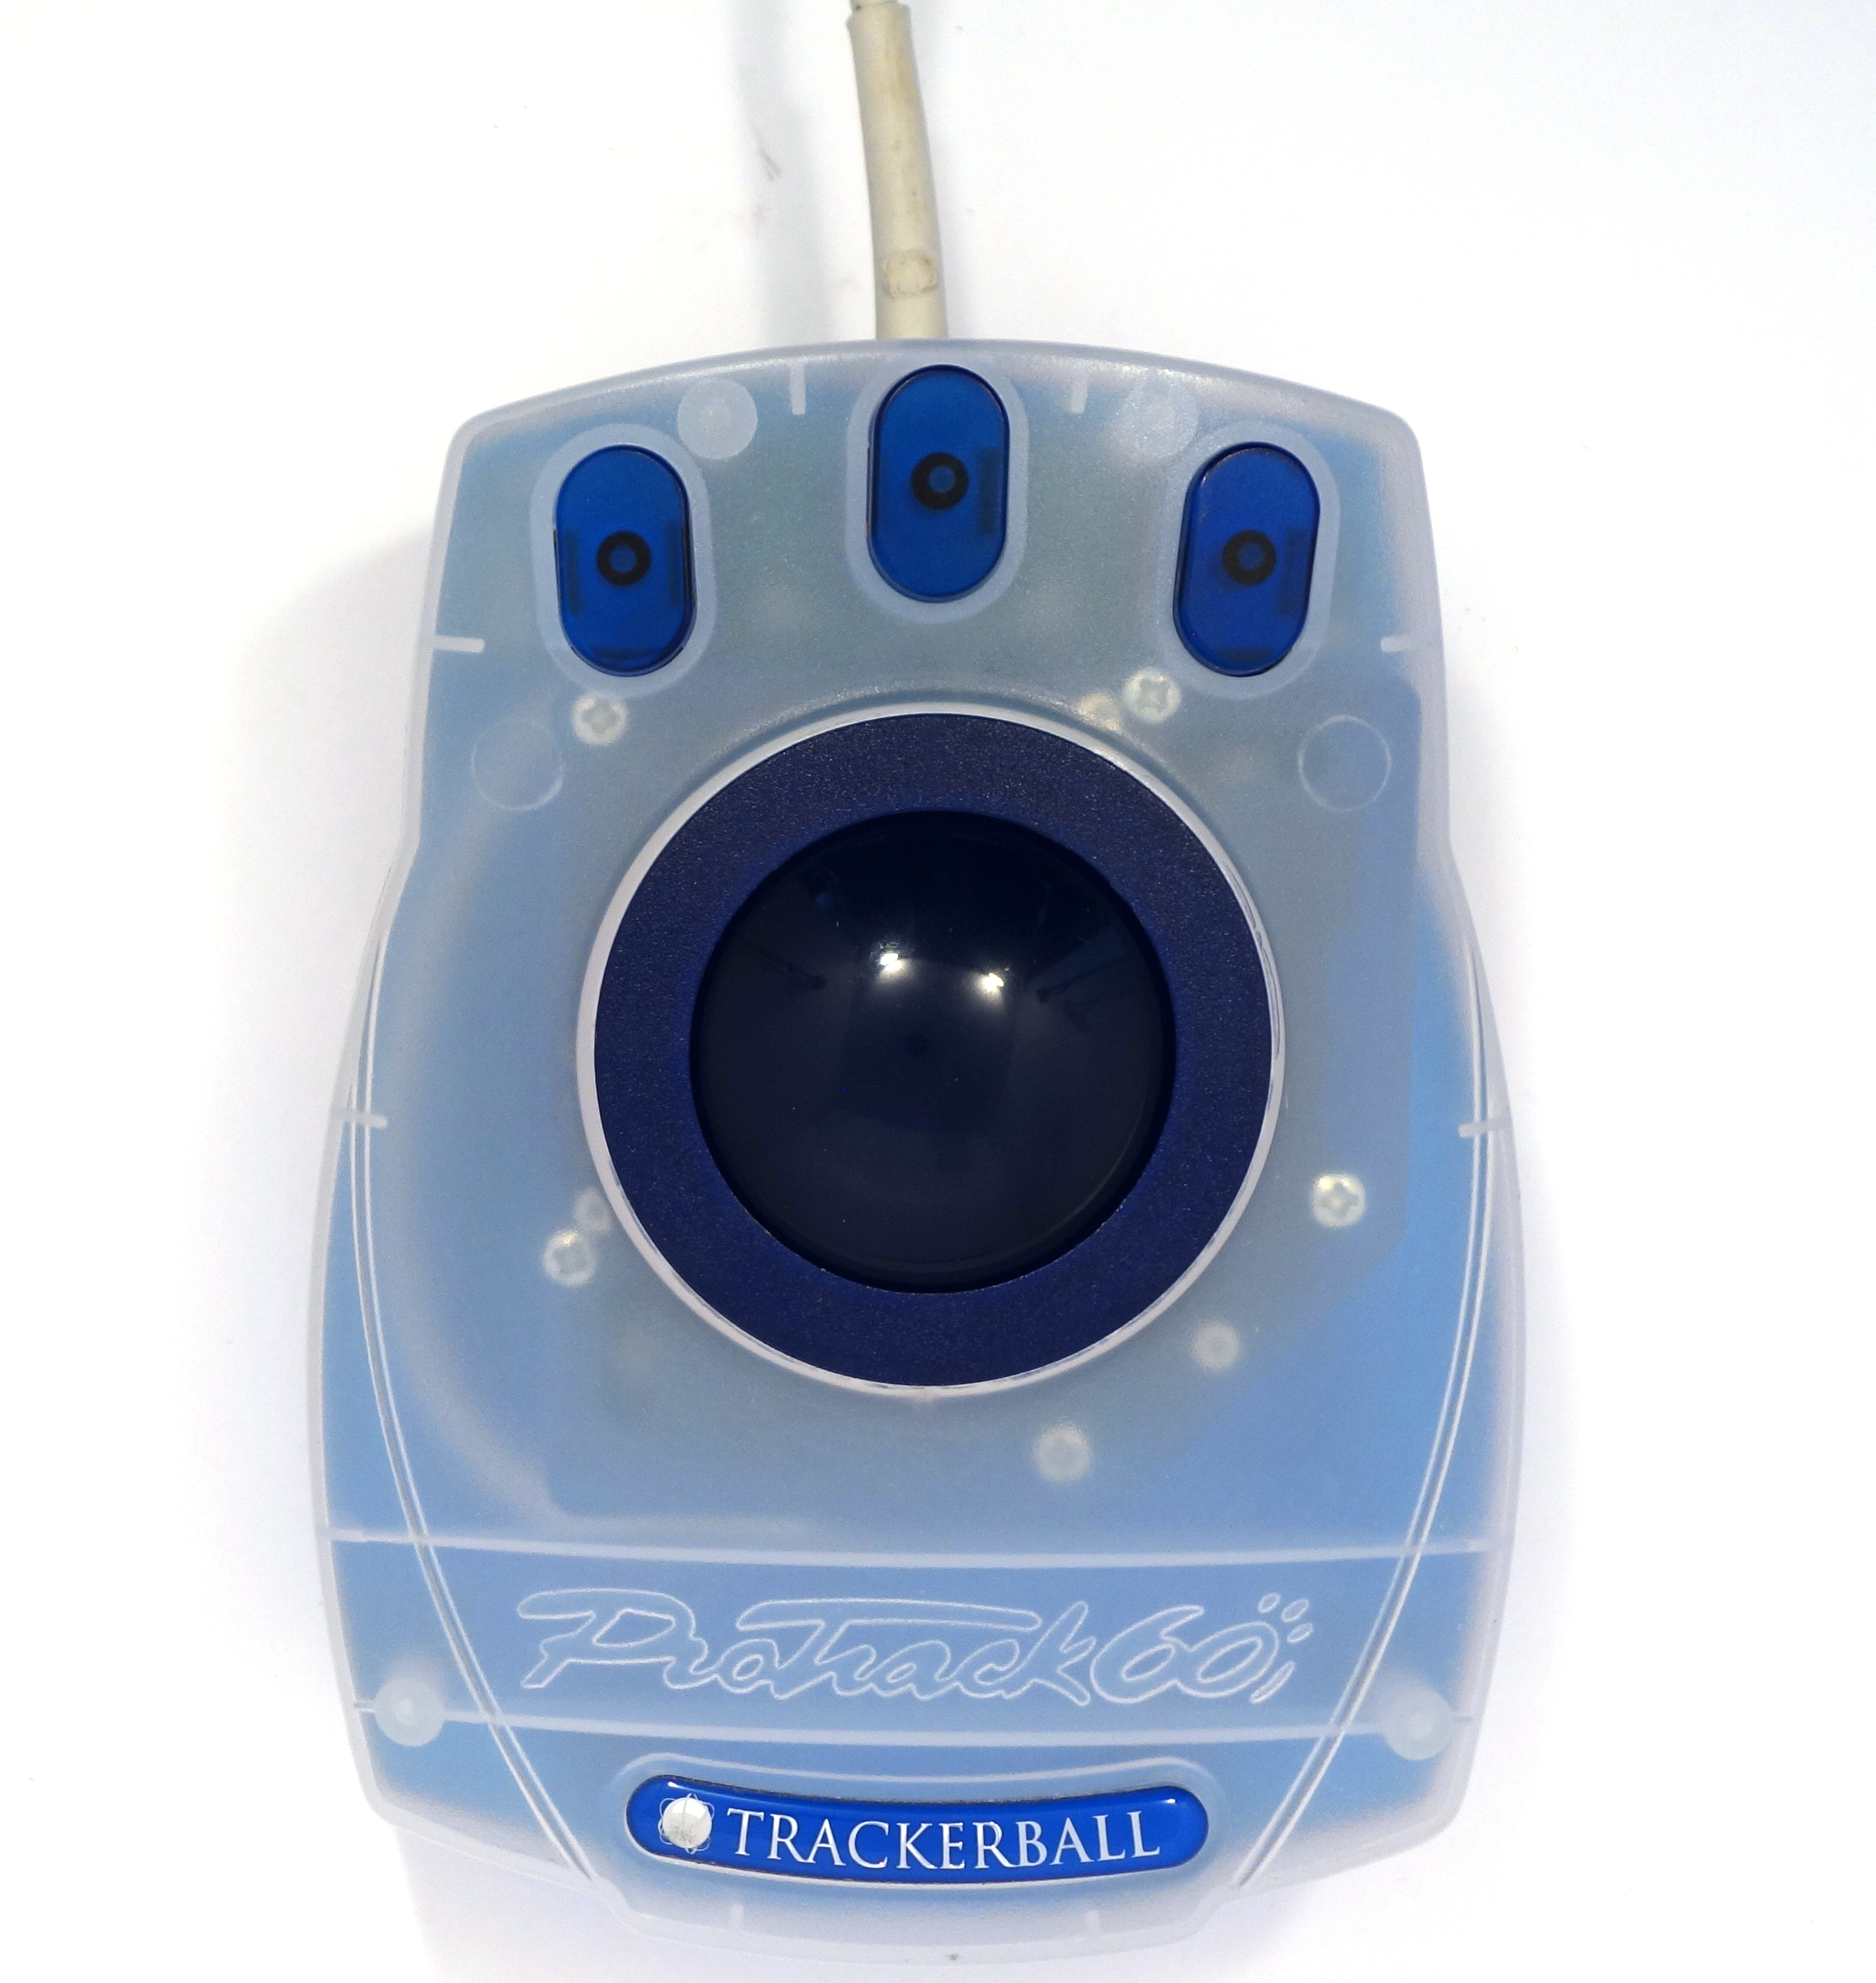
\includegraphics[scale=0.3]{1999_protrack_60i/monstr3_60.jpg}
    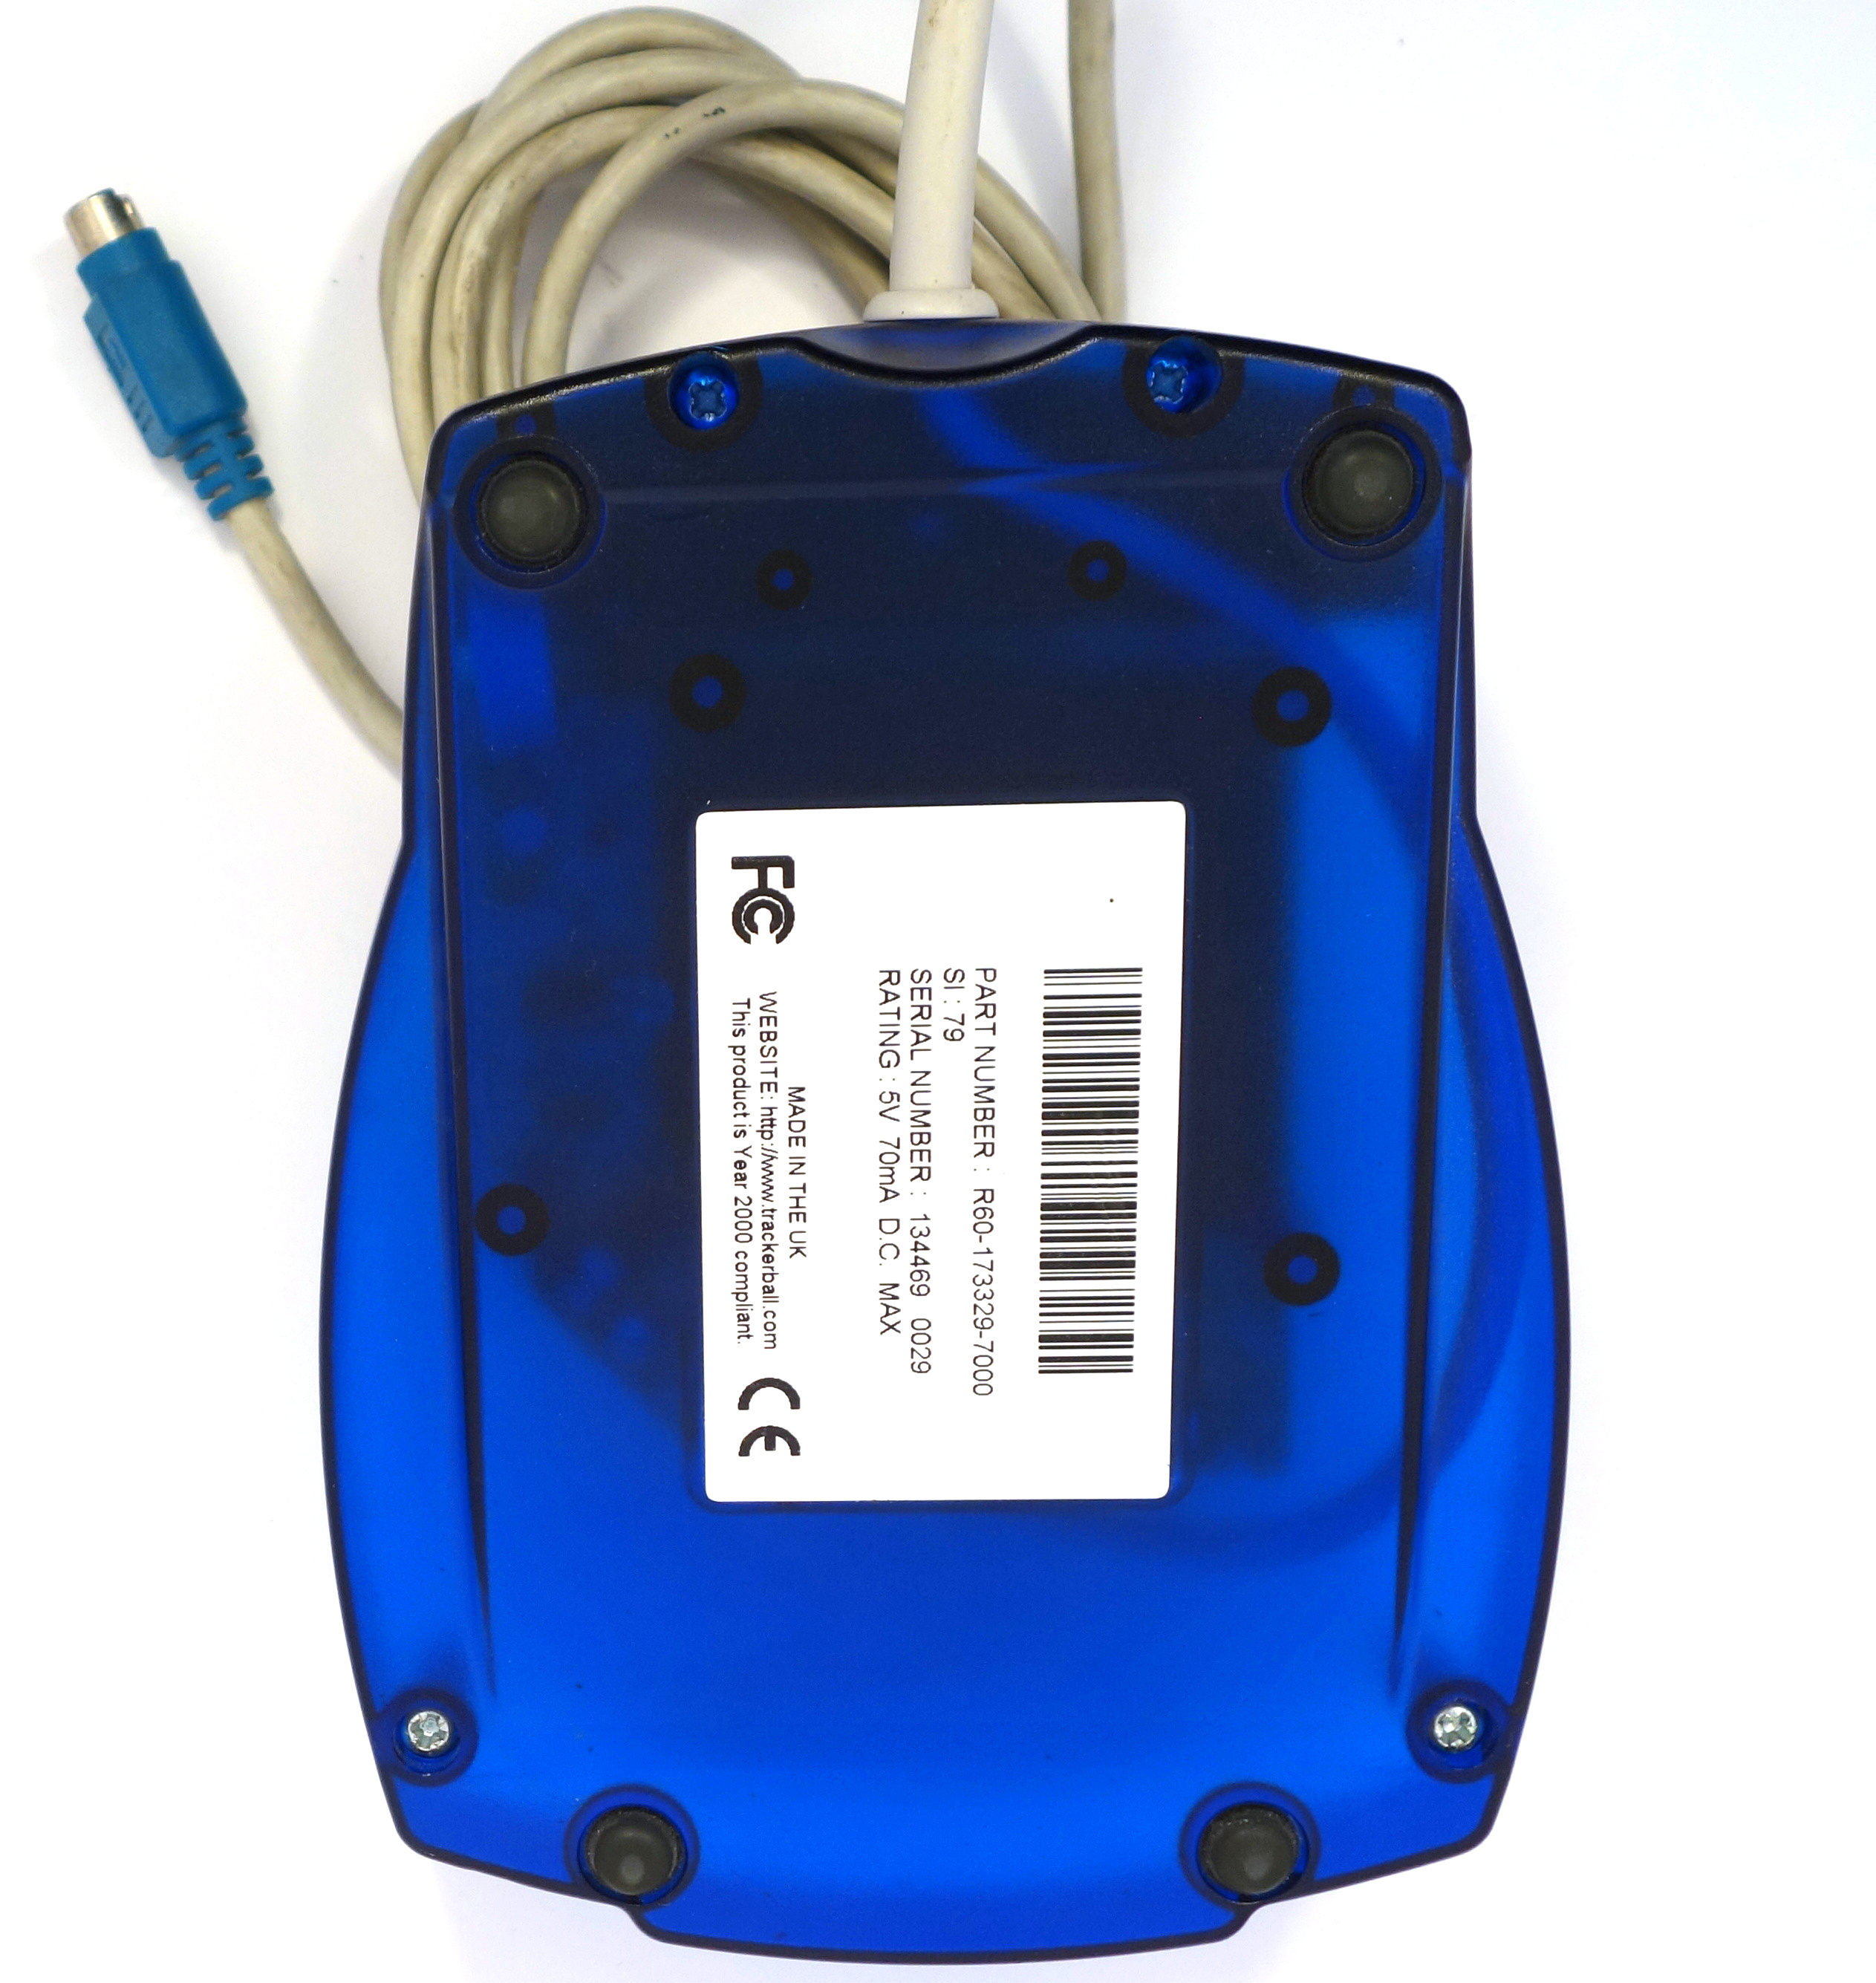
\includegraphics[scale=0.3]{1999_protrack_60i/monstr4_60.jpg}
    \caption{ProTrack 60i, вид сверху и снизу}
     \label{fig:ProTrack60iTopBottom}
\end{figure}

На нижней стенке корпуса присутствуют резиновые ножки, фиксирующие надёжное положение на поверности стола, и маркировка ProTrack 60i. Страной изготовления устройства является Великобритания.

\begin{figure}[h]
    \centering
    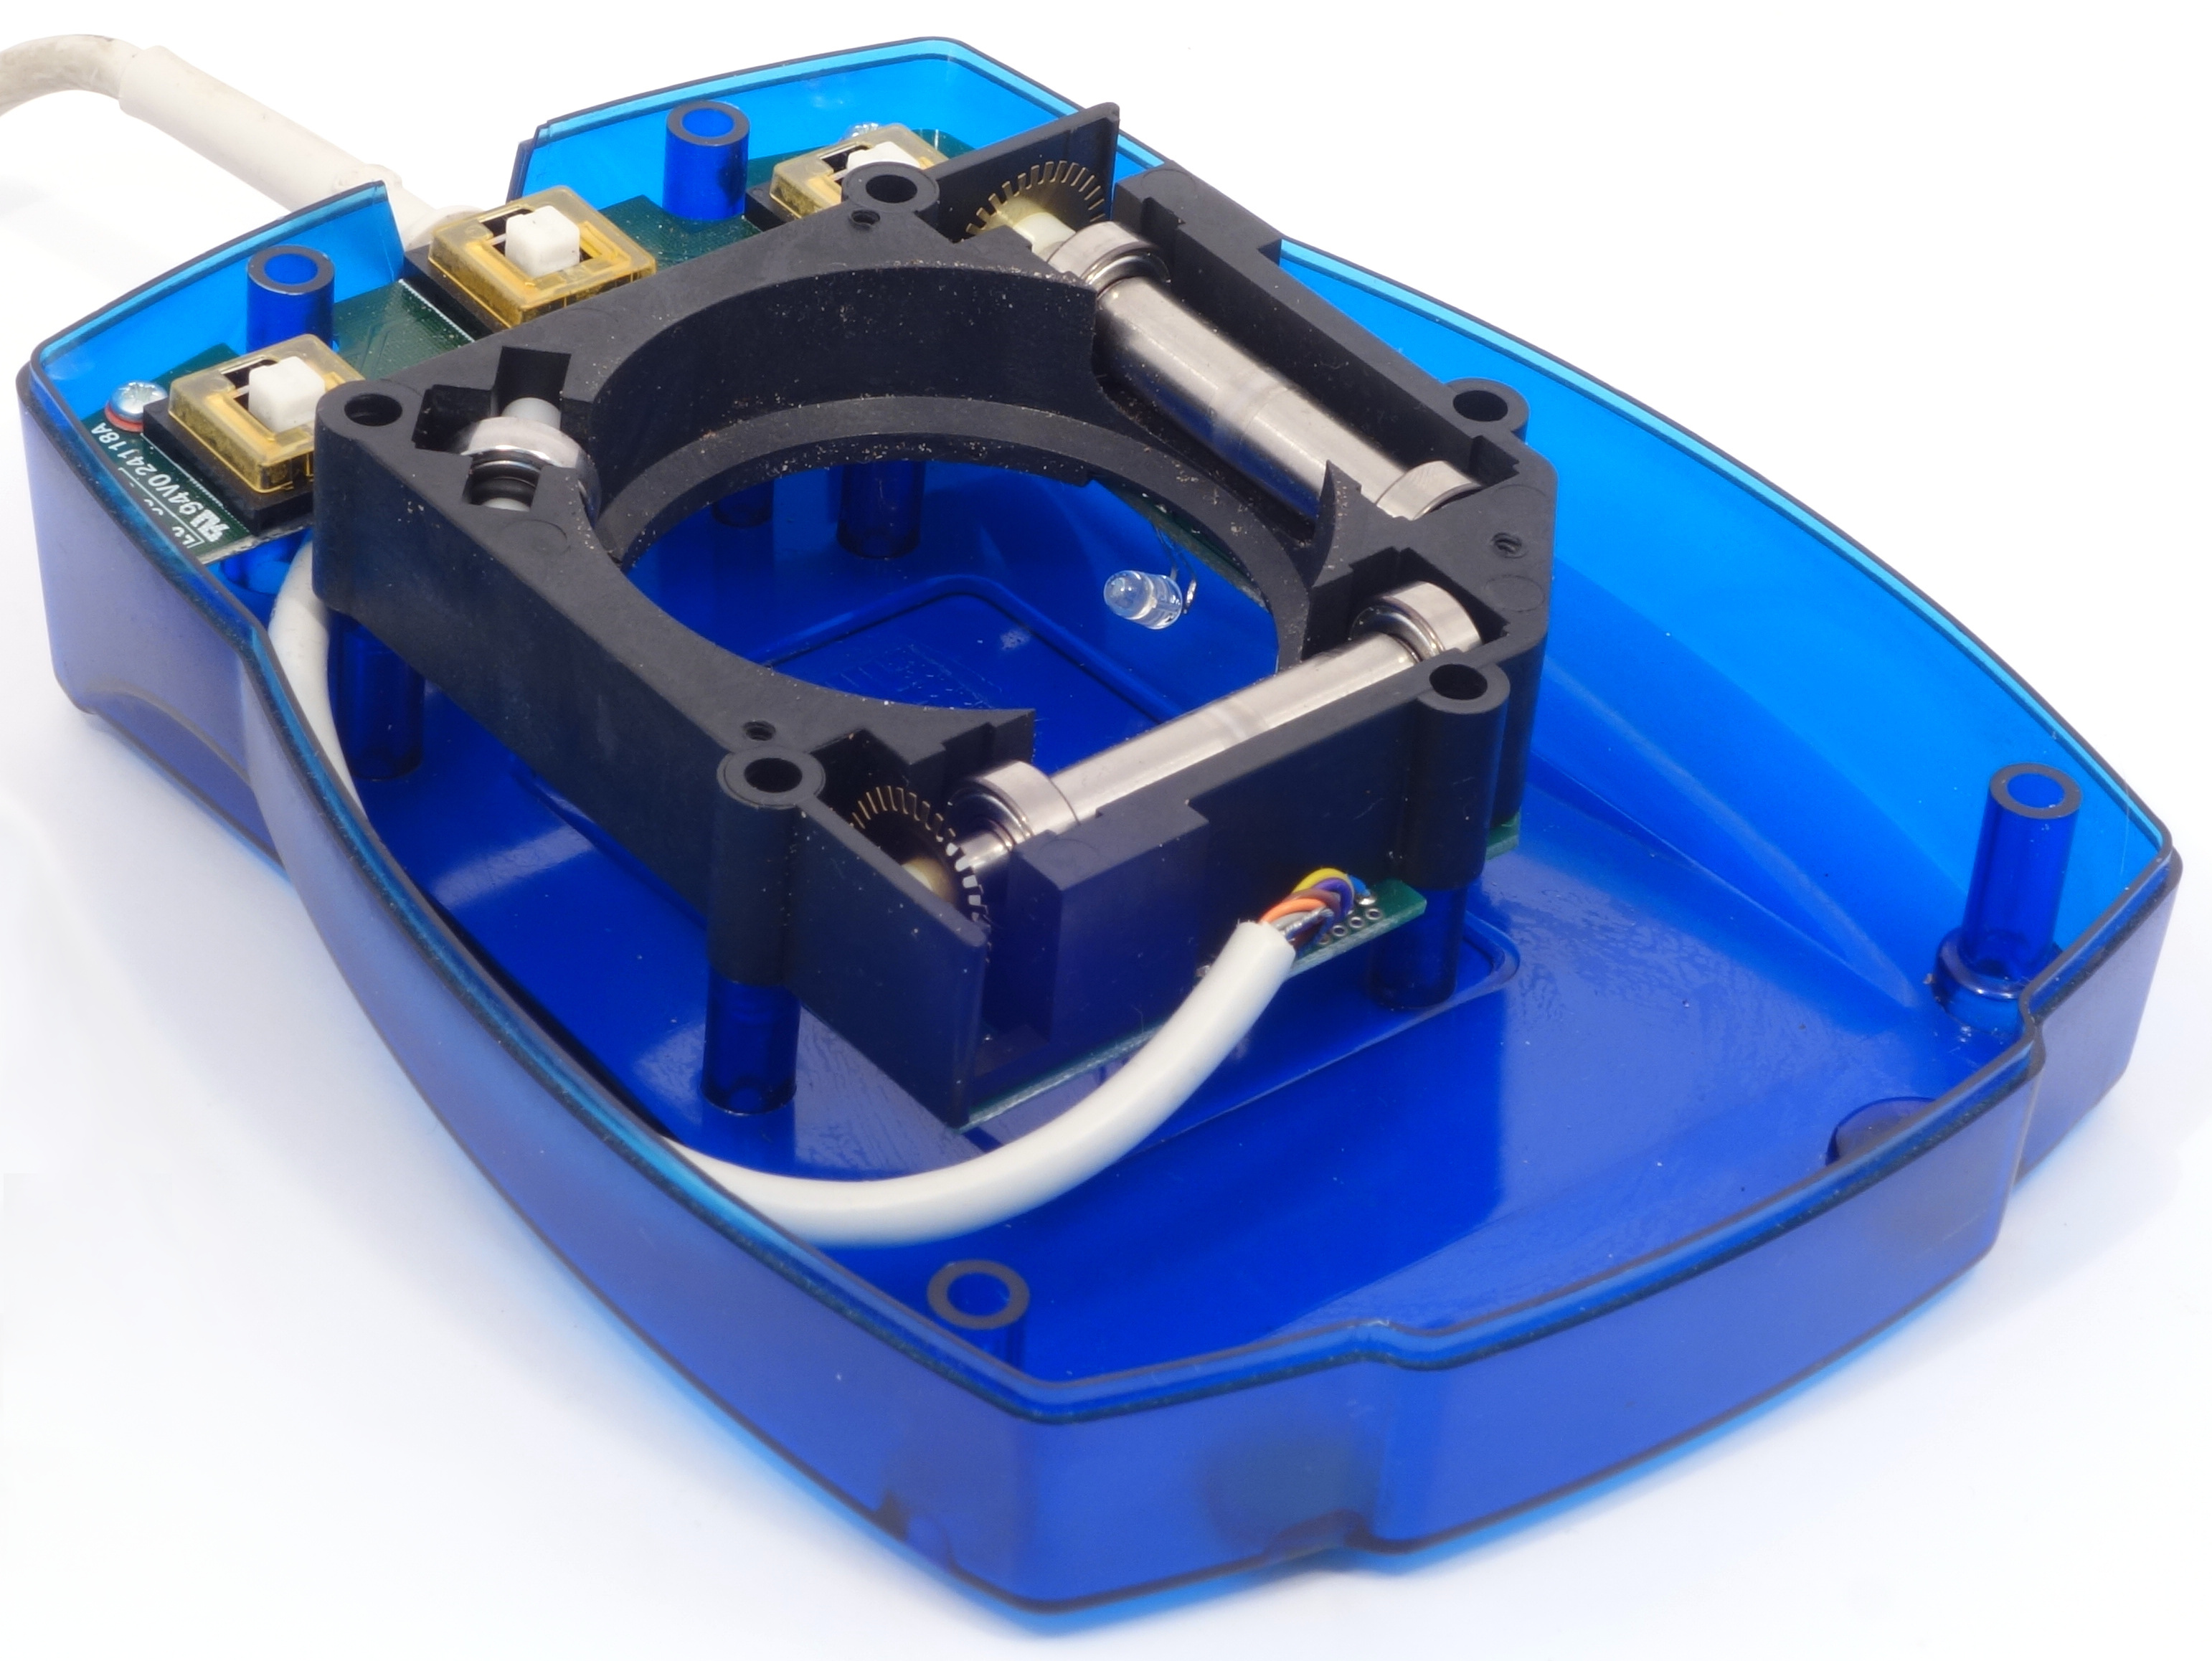
\includegraphics[scale=0.6]{1999_protrack_60i/razobr3_60.jpg}
    \caption{ProTrack 60i в разобранном состоянии}
    \label{fig:ProTrack60iInside}
\end{figure}

 Внутреннее устройство данного трекбола показано на рис. \ref{fig:ProTrack60iInside}. Как можно видеть,  трекбол выполнен по традиционной оптомеханической схеме, с дополнительным светодиодом, обеспечивающим подсветку шара. Также следует отметить, что ролики реализованы с использованием подшипников и валов из нержавеющей стали, предназначенных для того, чтобы обеспечить максимальную надежность и долговечность конструкции.
По всей видимости, извлечение шара для чистки трекбола невозможно без разборки корпуса.

\begin{thebibliography}{9}
\bibitem{history} History of Cursor Controls, innovators in trackball manufacturing \url{https://www.cursorcontrols.com/about/history/}
\bibitem{cursorcontrols} Cursor Controls Protrack 60 Industrial \url{https://web.archive.org/web/20010311155954/http://www.cursorcontrols.com/protrack60i.htm}
\bibitem{trackerball} The Trackerball Company - Products \url{https://web.archive.org/web/19990128124617/http://www.trackerball.com/PRODUCT.HTM}
\bibitem{trackballfan} Trackball Fan! Cursor Controls ProTrack 60i (R60i) \url{http://www.hykw.com/tbfan/reviews/protrack.shtml}
\end{thebibliography}
\end{document}
